%************************************************
\chapter{Introduction}\label{ch:introduction}
%************************************************

In recent years, we are witnessing an unprecedented level of presence of technology in our lives. Mobile phones are smarter every day, with computational power that overtakes desktop computers just a couple of years old. At the same time, these devices gain in ubiquity as they extend their functionality to wearable technology, e.g. wearable cameras, wireless earphones or smart watches. The cameras installed in these devices have seen a similar increase in presence, resolution, quality of the lenses and sensors, etc.

The combination of better cameras with improved processing and ubiquitous connectivity makes computer vision a crucial discipline that contributes important and very diverse applications, some of them having a special role in inclusivity and a positive impact in quality of life.

The diagram shown in Figure~\ref{fig:cv_dev_pipeline} illustrates the preliminary stages followed in computer vision prior to the development of an application. These are very common in research and entail the development of a prototype that is later refined with the use of data. 

Data is the cornerstone for learning and at the same time for parameter optimisation in many artificial intelligence fields. Within computer vision, data and in particular annotated data has driven research from the very origins. The availability of these annotated datasets has achieved a remarkable prominence with the organisation of systematic and objective challenges around the object recognition and detection topics that leveraged the massive proliferation of images and videos on the Internet (PASCAL VOC \cite{everingham2010pascal} and ImageNet \citep{Deng2009}), benchmarks that are becoming  more popular in other fields within computer vision such as navigation (NAVVIS \cite{Huitl2012} and SLAMbench \cite{nardi2014introducing}).

In recent years, Big Data, or the use of massive amounts of structured and unstructured data has made learning and prediction algorithms an extraordinarily important piece of the artificial intelligence puzzle. However, relying almost entirely in the use of data to solve the problem has sometimes caused the lost of perspective and very poor improvements on performance or none at all (\ref{}, \ref{}). What is more, the lack of understanding of the intrinsics of the problem has often seen important delays when solving the problem in question with their financial consequences. It is therefore important to keep developing core algorithms that help solve the problem by understanding what causes it. Often the solution is closer than what we think, and biology provides us with efficient models that solve the problem in an effective way. In particular in computer vision, models of the visual system have demonstrated being effective in key tasks such as object recognition and visual localisation \cite{lowe2004distinctive,milford2004ratslam}. 


\begin{figure}
\centering
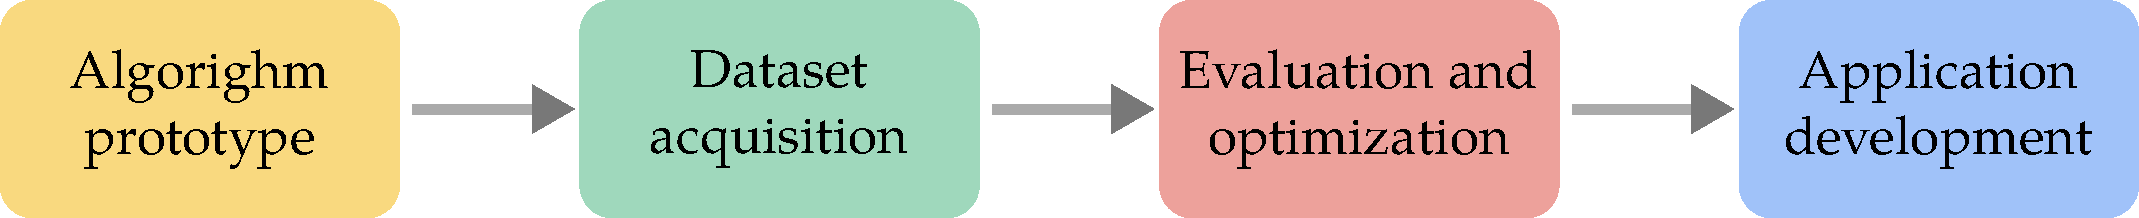
\includegraphics[width=\linewidth]{gfx/Chapter01/cv_dev_pipeline.pdf}
\caption{Stages in the development of a computer vision application. The development of an application in computer vision and similar artificial intelligence disciplines requires a different form of testing compared to the ones seen in standard software engineering toolchains. The use of databases and evaluation and optimisation stages prior to the development of the application complements the typical deterministic behaviour test suites.}
\label{fig:cv_dev_pipeline}
\end{figure}


This thesis represents 

\section{Organisation of the thesis}

The remainder of this dissertation is organised as follows: Chapter 2 presents our motivation on the acquisition of datasets and early work on appearance-based methods for visual localisation. Chapter 3 describes the SHORT dataset, a dataset for hand-held object recognition with an emphasis on the assistive context. Chapter 4 introduces our evaluation benchmark of descriptors for visual localisation. Chapter 5 presents our biologically inspired framework for visual localisation. In addition, we show experimental results of place-cells localisation  and a comparison with state-of-the-art SLAM. Chapter 6 describes our assistive vision-based localisation App that uses a wearable camera and a haptic feedback tablet to provide basic positional information. Finally in Chapter 7 we provide concluding remarks while summarising the main contributions of this dissertation and future work.


